\section{تحلیل علمی و کالبدشکافی ساختاری ماژول \lr{adaptive\_sparse\_attention}}
\label{sec:adaptive_sparse_attention}

\subsection*{بخش ۱: ایده محوری و چرایی معماری \lr{(Architectural Rationale)}}
توزیع احتمالاتی در مکانیزم خودتوجهی چندسره استاندارد \lr{(Multi-Head Attention - MHA)} به دلیل بهره‌گیری از عملگر سافت‌مکس چگال، مقادیر اکیداً مثبت را به تمامی نشانه‌های دنباله تخصیص می‌دهد ($\mathbf{A}_{ij} > 0, \forall i, j$). این فرمول‌بندی نمایی، دو نارسایی عمیق محاسباتی و ادراکی به همراه دارد: نخست تحمیل پیچیدگی درجه دوم $\mathcal{O}(N^2)$ در زمان و مصرف حافظه گرافیکی، و دوم تزریق مداوم آنتروپی زاید و نوفه آماری ناشی از تجمع وزن‌های کوچک نشانه‌های پس‌زمینه (نظیر نشانه‌های نشانه‌گذاری و کلمات دستوری کم‌اهمیت) به درون بردار بازنمایی نهایی توکن‌ها. تحلیل‌های تجربی بر روی فضاهای پنهان ترنسفورمر نشان داده است که وزن‌های مؤثر معنایی تنها بر روی زیرمجموعه بسیار کوچکی از جفت‌توکن‌ها تمرکز دارند و توزیع توجه در لایه‌های میانی و فوقانی ماهیتی شدیداً تنک \lr{(Sparse)} از خود بروز می‌دهد.

رویکردهای تنک‌سازی کلاسیک بر پایه‌های هندسی صلب نظیر پنجره‌های لغزان موضعی \lr{(Local Sliding Windows)} یا الگوهای ساختاریافته از پیش‌تعیین‌شده (مانند \lr{Longformer} و \lr{BigBird}) بنا شده‌اند. این الگوهای استاتیک، بدون توجه به محتوای سمانتیک، ساختار اتصال گراف توجه را محدود می‌کنند؛ در نتیجه، در پیوندهای معنایی دوربرد (مانند ارجاع ضمایر به مرجع در فواصل چندصد توکنی یا ارتباط فاعل و فعل در ساختارهای درهم‌تنیده)، الگوهای هندسی صلب دچار شکست کامل می‌شوند.

معماری \lr{adaptive\_sparse\_attention} با معرفی سازوکار گزینش تنک تطبیقی وابسته به محتوا \lr{(Content-Dependent Dynamic Top-K Routing)}، این چالش را بنیادین برطرف می‌سازد. در این ماژول، هر سر توجه به صورت مستقل و بر پایه انرژی ضرب داخلی پرس‌وجو--کلید \lr{(Query-Key Dot Product)}، بودجه نشانه‌های کلیدی فعال خود را مشخص می‌کند. نشانه‌های نامرتبط به طور صریح به $-\infty$ ماسک شده و از توزیع سافت‌مکس حذف می‌گردند که معادل وزن صفر قطعی در ماتریس توجه است.

چهار مؤلفه تحلیلی و مهندسی متمایز در طراحی این ماژول تعبیه شده است:
\begin{enumerate}
    \item \textbf{تخصیص بودجه تنک‌سازی متمایز برای انکودرها و دیکودرها:} در مدل‌های انکودر دوطرفه \lr{(Bidirectional Encoders)} مانند \lr{DistilBERT} و \lr{RoBERTa-base}، نشانه‌ها اطلاعات بافتی را از سرتاسر دنباله گردآوری می‌کنند؛ بنابراین، اعمال تنک‌سازی تهاجمی زودهنگام (مثلاً حذف ۵۰ درصدی) به سرعت شبکه‌های ادراکی را متلاشی می‌سازد. از این رو، بودجه تنک پیش‌فرض انکودرها به صورت محافظه‌کارانه بر روی \lr{0.1} (حذف ۱۰ درصد کم‌اهمیت‌ترین‌ها) تنظیم گردیده است. در نقطه مقابل، در دیکودرهای خودبازگشت \lr{(Autoregressive Decoders)} نظیر \lr{GPT-2} و \lr{Qwen3.5}، نرخ تنک‌سازی به \lr{0.5} (حذف ۵۰ درصد تاریخچه) ارتقا می‌یابد.
    \item \textbf{رعایت اصل عدم‌نشت علّی قبل از مرتب‌سازی \lr{(Pre-Sort Causal Masking)}:} در دیکودرها، چنانچه فیلتر بیشینه \lr{Top-K} پیش از اعمال ماسک مثلثی علّی \lr{(Causal Mask)} فراخوانی شود، توکن‌های آینده به دلیل انرژی اولیه بالا در گزینش وارد شده و سپس در مرحله ماسک علّی صفر می‌گردند؛ این پدیده موسوم به نشت علّی \lr{(Causal Data Leakage)}، توکن فعلی را از نشانه‌های معتبر گذشته محروم می‌سازد. ماژول حاضر با اعمال صریح ماسک علّی پیش از الگوریتم مرتب‌سازی، اصالت زمانی تولید توکن را تضمین می‌کند.
    \item \textbf{گریز از تله لایه‌نشانی \lr{(Escaping the Padding Trap)}:} در وظایف دسته‌بندی توالی به کمک مدل‌های علی که ورودی‌ها از سمت راست لایه‌نشانی \lr{(Right-Padded)} می‌شوند، توکن نهایی دسته‌بندی در فاصله‌ای دور از نشانه‌های اصلی متن قرار می‌گیرد. مکانیزم‌های پنجره موضعی (نظیر \lr{Adaptive Span}) در این سناریو به طور کامل در میان توکن‌های تهی به دام می‌افتند. در مقابل، مکانیزم تنک تطبیقی جهانی \lr{(Global Dynamic Top-K)} بدون محدودیت مکانی، برترین کلیدها را از کل طول دنباله استخراج کرده و مسیر گرادیان مستقیم به سرنخ‌های متنی ابتدای جمله باز می‌دارد.
    \item \textbf{تثبیت گرادیان از طریق انجماد لاجیت تنک‌سازی و به‌کارگیری آداپتورهای کم‌رتبه \lr{(LoRA)}:} تابع گزینش گسسته رتبه برتر فاقد مشتق‌پذیری هموار است ($\nabla_k = 0$). برای ممانعت از پرش‌های ناگهانی گرادیان و واگرایی فرآیند بازیابی، پارامترهای لاجیت تنک‌سازی هر سر \lr{(sparsity\_logits)} به عنوان فراپارامتر ثابت منجمد شده \lr{(requires\_grad = False)} و تطبیق فضاهای برداری منحصراً توسط آداپتورهای \lr{LoRALinear} در طول لایه‌های پروجکشن صورت می‌پذیرد.
\end{enumerate}

\subsection*{بخش ۲: فرمولبندی ریاضی و مبانی نظری \lr{(Mathematical Formulation)}}
فرض کنید تانسور فعال‌سازی ورودی پرس‌وجو به صورت $\mathbf{X} \in \mathbb{R}^{B \times N_q \times D}$ و تانسور ورودی کلید-مقدار متناظر به صورت $\mathbf{X}_{kv} \in \mathbb{R}^{B \times N_k \times D}$ تعریف شوند، که در آن $B$ اندازه دسته، $N_q$ طول دنباله پرس‌وجو، $N_k$ طول دنباله کلید و $D$ بعد پنهان مدل است.

\paragraph{۱. نگاشت‌های خطی مجهز به آداپتورهای کم‌رتبه \lr{(LoRA Projections)}:}
تانسورهای ورودی توسط نگاشت‌های خطی با پارامترهای پایه منجمد $\mathbf{W}_0$ و شاخه‌های سازگار کم‌رتبه به فضاهای پرس‌وجو، کلید و مقدار نگاشت می‌شوند:
\begin{align}
\mathbf{Q}_{\text{flat}} &= \mathbf{X} \mathbf{W}_{0, Q}^\top + \frac{\alpha_{\text{lora}}}{r_{\text{lora}}} (\mathbf{X} \mathbf{A}_Q^\top) \mathbf{B}_Q^\top + \mathbf{b}_Q \in \mathbb{R}^{B \times N_q \times (H \cdot d)} \\
\mathbf{K}_{\text{flat}} &= \mathbf{X}_{kv} \mathbf{W}_{0, K}^\top + \frac{\alpha_{\text{lora}}}{r_{\text{lora}}} (\mathbf{X}_{kv} \mathbf{A}_K^\top) \mathbf{B}_K^\top + \mathbf{b}_K \in \mathbb{R}^{B \times N_k \times (H_{kv} \cdot d)} \\
\mathbf{V}_{\text{flat}} &= \mathbf{X}_{kv} \mathbf{W}_{0, V}^\top + \frac{\alpha_{\text{lora}}}{r_{\text{lora}}} (\mathbf{X}_{kv} \mathbf{A}_V^\top) \mathbf{B}_V^\top + \mathbf{b}_V \in \mathbb{R}^{B \times N_k \times (H_{kv} \cdot d)}
\end{align}
که در آن $H$ تعداد سرهای پرس‌وجو، $H_{kv}$ تعداد سرهای کلید-مقدار، $d$ بعد هر سر ($D = H \cdot d$)، $r_{\text{lora}}$ رتبه آداپتور، $\alpha_{\text{lora}}$ ضریب مقیاس‌بندی و $\mathbf{A} \in \mathbb{R}^{r_{\text{lora}} \times D}$ و $\mathbf{B} \in \mathbb{R}^{D_{\text{out}} \times r_{\text{lora}}}$ ماتریس‌های کم‌رتبه هستند.

\paragraph{۲. بازآرایی ساختار چندسره و کدگذاری موقعیت چرخشی \lr{(RoPE)}:}
تانسورها به ابعاد ۴-بعدی تفکیک شده و دوران مکانی بر روی ابعاد سرها اعمال می‌گردد:
\begin{align}
\mathbf{Q} &= \operatorname{transpose}(\operatorname{view}(\mathbf{Q}_{\text{flat}}, [B, N_q, H, d]), 1, 2) \in \mathbb{R}^{B \times H \times N_q \times d} \\
\mathbf{K} &= \operatorname{transpose}(\operatorname{view}(\mathbf{K}_{\text{flat}}, [B, N_k, H_{kv}, d]), 1, 2) \in \mathbb{R}^{B \times H_{kv} \times N_k \times d} \\
\mathbf{V} &= \operatorname{transpose}(\operatorname{view}(\mathbf{V}_{\text{flat}}, [B, N_k, H_{kv}, d]), 1, 2) \in \mathbb{R}^{B \times H_{kv} \times N_k \times d}
\end{align}
عملگر دوران مکانی چرخشی \lr{(Rotary Position Embedding - RoPE)} برای جفت بردارهای $\mathbf{q}_m, \mathbf{k}_n \in \mathbb{R}^d$ در موقعیت‌های زمانی $m$ و $n$ به فرم زیر است:
\begin{equation}
\tilde{\mathbf{q}}_m = \mathbf{q}_m \odot \cos(m \boldsymbol{\theta}) + \operatorname{rotate\_half}(\mathbf{q}_m) \odot \sin(m \boldsymbol{\theta})
\end{equation}
\begin{equation}
\tilde{\mathbf{k}}_n = \mathbf{k}_n \odot \cos(n \boldsymbol{\theta}) + \operatorname{rotate\_half}(\mathbf{k}_n) \odot \sin(n \boldsymbol{\theta})
\end{equation}
که در آن $\boldsymbol{\theta} = \{\theta_i = 10000^{-2(i-1)/d}\}_{i=1}^{d/2}$ فرکانس‌های مبنا بوده و $\operatorname{rotate\_half}(\mathbf{x}) = [-\mathbf{x}_{d/2:d}, \mathbf{x}_{0:d/2}]$ است.

چنانچه مدل از سازوکار توجه پرس‌وجوی گروهی \lr{(GQA)} بهره ببرد ($H > H_{kv}$)، تانسورهای کلید و مقدار با نرخ تکرار $G = H / H_{kv}$ در راستای بعد سرها همتاسازی می‌شوند:
\begin{equation}
\mathbf{K} \leftarrow \operatorname{repeat\_kv}(\mathbf{K}, G) \in \mathbb{R}^{B \times H \times N_k \times d}, \quad \mathbf{V} \leftarrow \operatorname{repeat\_kv}(\mathbf{V}, G) \in \mathbb{R}^{B \times H \times N_k \times d}
\end{equation}

\paragraph{۳. قطعه‌بندی پرس‌وجو و محاسبه ماتریس خام امتیازات:}
برای بهینه‌سازی ترافیک ثبات‌ها و حفظ بافرها در حافظه نهان، محاسبات بر روی قطعات پرس‌وجو با اندازه ثابت $C_q = 64$ انجام می‌پذیرد. برای قطعه $c \in \{0, \dots, \lceil N_q / C_q \rceil - 1\}$:
\begin{equation}
\mathbf{S}_c = \frac{\mathbf{Q}[:, :, q_{\text{start}}:q_{\text{end}}, :] \cdot \mathbf{K}^\top}{\sqrt{d}} \in \mathbb{R}^{B \times H \times C_q \times N_k}
\end{equation}
در صورت وجود انحراف موقعیت نسبی \lr{(Relative Position Bias)} نظیر مدل \lr{T5}:
\begin{equation}
\mathbf{S}_c \leftarrow \mathbf{S}_c + \mathbf{B}_{\text{rel}}[:, :, q_{\text{start}}:q_{\text{end}}, :]
\end{equation}

\paragraph{۴. اعمال ماسک لایه‌نشانی و ماسک علّی پیش از گزینش تنک:}
نخست نشانه‌های لایه‌نشانی نامعتبر حذف می‌گردند:
\begin{equation}
S_{c, b, h, i, j} \leftarrow \begin{cases} S_{c, b, h, i, j} & \text{if } \mathbf{M}_{\text{valid}, b, j} = 1 \\ -10000.0 & \text{if } \mathbf{M}_{\text{valid}, b, j} = 0 \end{cases}
\end{equation}
در صورت فعال بودن حالت دیکودر خودبازگشت، ماسک مثلثی پایینی علّی اعمال می‌گردد:
\begin{equation}
S_{c, b, h, i, j} \leftarrow \begin{cases} S_{c, b, h, i, j} & \text{if } j \le (q_{\text{start}} + i) \\ -10000.0 & \text{if } j > (q_{\text{start}} + i) \end{cases}
\end{equation}

\paragraph{۵. گزینش برداری آستانه پویای \lr{Top-K} و تنک‌سازی:}
به ازای هر سر توجه $h \in \{1, \dots, H\}$، نسبت تنک‌سازی $\gamma_h$ و تعداد نشانه‌های مجاز $k_h$ تعیین می‌شود:
\begin{equation}
\gamma_h = \operatorname{clamp}\left(\sigma(\omega_h), 0.0, 0.95\right), \quad \omega_h \in \mathbb{R} \text{ (frozen sparsity logit)}
\end{equation}
\begin{equation}
k_h = \operatorname{clamp}\left(\left\lfloor (1.0 - \gamma_h) \cdot N_k \right\rfloor, 1, N_k\right)
\end{equation}
ماتریس نمرات در امتداد بعد کلیدها ($N_k$) به صورت نزولی مرتب‌سازی موازی می‌شود:
\begin{equation}
\mathbf{S}_{\text{sorted}, c} = \operatorname{SortDesc}(\mathbf{S}_c, \text{dim}=-1) \in \mathbb{R}^{B \times H \times C_q \times N_k}
\end{equation}
سپس آستانه قطع سطرها $\tau_{b, h, i}$ با عملگر واکشی برداری \lr{(Vectorized Gather)} در ایندکس $k_h - 1$ استخراج می‌گردد:
\begin{equation}
\tau_{b, h, i} = \mathbf{S}_{\text{sorted}, c}[b, h, i, k_h - 1] \in \mathbb{R}
\end{equation}
ماسک‌گذاری صریح درایه‌های پایین‌تر از آستانه:
\begin{equation}
\tilde{S}_{c, b, h, i, j} = \begin{cases} S_{c, b, h, i, j} & \text{if } S_{c, b, h, i, j} \ge \tau_{b, h, i} \\ -10000.0 & \text{if } S_{c, b, h, i, j} < \tau_{b, h, i} \end{cases}
\end{equation}

\paragraph{۶. نرمال‌سازی سافت‌مکس تنک و تجمیع زمینه:}
ماتریس وزن‌های توجه تنک $\mathbf{A}_c$ و تانسور خروجی قطعه $\mathbf{O}_c$ ارزیابی می‌گردد:
\begin{equation}
\mathbf{A}_c = \operatorname{Dropout}\left(\operatorname{Softmax}(\tilde{\mathbf{S}}_c, \text{dim}=-1)\right) \in \mathbb{R}^{B \times H \times C_q \times N_k}
\end{equation}
\begin{equation}
\mathbf{O}_c = \mathbf{A}_c \cdot \mathbf{V} \in \mathbb{R}^{B \times H \times C_q \times d}
\end{equation}
قطعات خروجی در امتداد طول دنباله به هم متصل شده و پس از بازآرایی، از لایه پروجکشن خروجی عبور می‌کنند:
\begin{equation}
\mathbf{O}_{\text{ctx}} = \operatorname{Concat}_{c=0}^{\lceil N_q / C_q \rceil - 1}(\mathbf{O}_c) \in \mathbb{R}^{B \times H \times N_q \times d} \xrightarrow{\operatorname{view}} \mathbb{R}^{B \times N_q \times (H \cdot d)}
\end{equation}
\begin{equation}
\mathbf{Y} = \left(\operatorname{LoRA-Linear}_O(\mathbf{O}_{\text{ctx}})\right) \cdot \alpha_{\text{scale}} \in \mathbb{R}^{B \times N_q \times D}
\end{equation}

\paragraph{۷. تحلیل پیچیدگی محاسباتی و حافظه:}
\begin{itemize}
    \item \textbf{پیچیدگی زمانی \lr{(Time Complexity)}:} ضرب ماتریسی پروجکشن‌ها معادل $\mathcal{O}(B N_q D^2)$ است. محاسبه ضرب قطعه‌ای $\mathbf{Q}_c \mathbf{K}^\top$ نیازمند $\mathcal{O}(B H N_q N_k d)$ عملیات ممیز شناور است. مرتب‌سازی موازی در امتداد بعد کلید دارای پیچیدگی $\mathcal{O}(B H N_q N_k \log N_k)$ بوده که با الگوریتم‌های انتخاب سریع \lr{(QuickSelect / Min-Heap)} بر روی سخت‌افزار تا $\mathcal{O}(B H N_q N_k)$ تقلیل می‌یابد. ضرب تنک نهایی $\mathbf{A}_c \mathbf{V}$ در صورت بهره‌گیری از هسته‌های فشرده تنک \lr{(CSR)} به $\mathcal{O}(B H N_q \bar{k} d)$ کاهش می‌یابد که در آن $\bar{k} = \frac{1}{H}\sum_h k_h \ll N_k$ است.
    \item \textbf{پیچیدگی مکانی \lr{(Space Complexity)}:} بر خلاف توجه استاندارد که نیازمند نگه‌داری ماتریس کامل $[B, H, N_q, N_k]$ در حافظه سراسری است، قطعه‌بندی پرس‌وجو با اندازه $C_q = 64$ سقف حافظه فعال‌سازی موقت را به $\mathcal{O}(B H C_q N_k)$ محدود می‌سازد که مقیاس‌بندی خطی نسبت به طول دنباله پرس‌وجو را در طول گذر پیشرو به ارمغان می‌آورد.
\end{itemize}

\subsection*{بخش ۳: کالبدشکافی سورسکد و ردگیری تانسورها \lr{(Source Code \& Tensor Trace)}}
ماژول \lr{adaptive\_sparse\_attention.py} در چارچوب یک کلاس صنعتی مقاوم‌سازی‌شده \lr{(Production-Hardened)} سازمان‌دهی شده است.

\paragraph{۱. سلسله‌مراتب کلاس‌ها و ثبت در رجیستری:}
کلاس اصلی \lr{AdaptiveSparseAttention} از کلاس پایه \lr{BaseAttention} ارث‌بری می‌کند و به کمک دکوراتور \lr{@ATTENTION\_REGISTRY.register} تحت چهار نام مستعار ثبت گردیده است:
\begin{itemize}
    \item \lr{"adaptive\_sparse"}
    \item \lr{"adaptive\_sparse\_attention"}
    \item \lr{"adaptive\_sparse\_attn"}
    \item \lr{"adaptive\_sparse\_attention\_attention"}
\end{itemize}
کلاس کمکی \lr{LoRALinear} مسئولیت خطی‌سازی وزن‌ها همراه با شاخه‌های کم‌مرتبه قابل انجماد را بر عهده دارد.

\paragraph{۲. استخراج و انتقال وزن‌ها \lr{(copy\_weights)}:}
متد \lr{copy\_weights} از یک پروتکل پنج‌مرحله‌ای قوی بهره می‌برد:
\begin{itemize}
    \item استخراج لایه‌های استاندارد هاگینگ‌فیس از طریق کلاس کمکی \lr{UniversalAdapter.get\_weight\_bias}.
    \item پشتیبانی کامل از لایه‌های ترکیب‌شده \lr{Conv1D} در مدل \lr{GPT-2} \lr{(c\_attn, c\_proj)} از طریق ترانهاده‌سازی ابعاد و تفکیک سه‌گانه وزن‌ها و بایاس‌ها به $Q$ و $K$ و $V$.
    \item تشخیص انکودرهای تودرتو \lr{(Nested Encoders)} در مدل‌های \lr{RoBERTa} و \lr{BERT} \lr{(BertSelfAttention, RobertaSelfAttention)} که فاقد لایه پروجکشن خروجی درون‌بسته‌ای هستند؛ در این حالت، فلگ \lr{is\_nested\_encoder = True} فعال شده و ماتریس پروجکشن خروجی با ماتریس همانی مقداردهی می‌شود تا از اعوجاج در بازنمایی جلوگیری گردد.
    \item ارزیابی شرایط نرم فروبنیوس ($\|\mathbf{W}\|_F \ge 10^{-4}$) بر روی تمامی قطعات استخراج‌شده جهت اطمینان از عدم بارگذاری ماتریس‌های تهی یا مقادیر عددی فاسد.
    \item انجماد وزن‌های مبنا در صورت فعال بودن رتبه آداپتور ($\text{lora\_rank} > 0$).
\end{itemize}

\paragraph{۳. جدول ردگیری گام‌به‌گام تانسورها \lr{(Tensor Shape Trace)}:}
جدول \ref{tab:tensor_trace_adaptive_sparse} دگرگونی ابعاد تانسورها را در طول خط لوله محاسباتی ماژول با فرض ابعاد تجربی $B=8$، $N=512$، $D=768$، $H=12$، $d=64$ و اندازه قطعه $C_q=64$ تشریح می‌کند.

\begin{table}[htbp]
\centering
\small
\caption{ردگیری گام‌به‌گام دگرگونی ابعاد تانسورها در ماژول \lr{adaptive\_sparse\_attention}}
\label{tab:tensor_trace_adaptive_sparse}
\begin{tabular}{clll}
\hline
\textbf{گام} & \textbf{عملگر محاسباتی} & \textbf{ابعاد تانسور خروجی} & \textbf{توضیحات فنی} \\
\hline
۱ & تانسور ورودی $\mathbf{X}$ & $[8, 512, 768]$ & بازنمایی پنهان توکن‌های دسته \\
۲ & پروجکشن‌های خطی با \lr{LoRA} & $[8, 512, 768]$ & اعمال نگاشت‌های خطی بر روی $Q, K, V$ \\
۳ & تفکیک چندسره و ترانهاده & $[8, 12, 512, 64]$ & تشکیل تانسورهای ۴-بعدی $[B, H, N, d]$ \\
۴ & اعمال نگاشت چرخشی \lr{RoPE} & $[8, 12, 512, 64]$ & اعمال تابع \lr{apply\_rotary\_pos\_emb} \\
۵ & همتاسازی کلید و مقدار \lr{(GQA)} & $[8, 12, 512, 64]$ & تکرار سرها در صورت نیاز ($H > H_{kv}$) \\
۶ & برش قطعه پرس‌وجو $\mathbf{Q}_c$ & $[8, 12, 64, 64]$ & قطعه‌بندی در راستای طول دنباله ($C_q = 64$) \\
۷ & محاسبه خام امتیازات $\mathbf{S}_c$ & $[8, 12, 64, 512]$ & ضرب داخلی $\mathbf{Q}_c \mathbf{K}^\top / \sqrt{d}$ \\
۸ & اعمال ماسک علّی (در دیکودر) & $[8, 12, 64, 512]$ & پر کردن درایه‌های آینده با $-10000.0$ \\
۹ & مرتب‌سازی نزولی برداری & $[8, 12, 64, 512]$ & فراخوانی تابع موازی \lr{torch.sort} \\
۱۰ & استخراج آستانه $\tau_{b, h, i}$ & $[8, 12, 64, 1]$ & عملگر \lr{torch.gather} در ایندکس $k_h - 1$ \\
۱۱ & فیلترینگ تنک پویا & $[8, 12, 64, 512]$ & ماسک‌گذاری امتیازات کمتر از $\tau$ \\
۱۲ & نرمال‌سازی سافت‌مکس و دراپ‌اوت & $[8, 12, 64, 512]$ & تولید ماتریس تنک احتمالات $\mathbf{A}_c$ \\
۱۳ & تجمیع زمینه قطعه $\mathbf{A}_c \mathbf{V}$ & $[8, 12, 64, 64]$ & ضرب ماتریسی در مقادیر مربوطه \\
۱۴ & اتصال قطعات و بازآرایی پیوسته & $[8, 512, 768]$ & تجمیع قطعات و تبدیل به تانسور یکپارچه \\
۱۵ & پروجکشن نهایی و مقیاس‌گذاری & $[8, 512, 768]$ & اعمال لایه \lr{out\_proj} و ضرب در $\alpha_{\text{scale}}$ \\
\hline
\end{tabular}
\end{table}

\paragraph{۴. جریان داده و دیاگرام ساختاری:}
جریان داده تانسوری و فرآیند تصمیم‌گیری آستانه تنک در شکل \ref{fig:arch_adaptive_sparse_attention} به تصویر کشیده شده است.

\begin{figure}[htbp]
\centering
\begin{tikzpicture}[
    scale=0.75, every node/.style={scale=0.75},
    node distance=0.9cm, auto,
    inb/.style={rectangle, draw=blue!70, fill=blue!12, rounded corners=4pt, align=center, text centered, minimum height=0.85cm},
    matmul/.style={circle, draw=orange!80, fill=orange!18, align=center, text centered, minimum size=0.85cm},
    thresh/.style={diamond, draw=purple!80, fill=purple!15, align=center, text centered, minimum size=0.9cm},
    sparse/.style={rectangle, draw=red!75, fill=red!15, rounded corners=4pt, align=center, text centered, minimum height=0.85cm},
    outb/.style={rectangle, draw=teal!80, fill=teal!15, rounded corners=4pt, align=center, text centered, minimum height=0.85cm}
]
    \node [inb] (input) {ورودی $\mathbf{X} \in \mathbb{R}^{B \times N \times D}$};
    \node [matmul, right=0.8cm of input] (dot) {$\frac{\mathbf{Q}_c\mathbf{K}^\top}{\sqrt{d}}$};
    \node [thresh, right=0.8cm of dot] (tau) {تعیین آستانه $\tau(\mathbf{S}_c)$};
    \node [sparse, right=0.8cm of tau] (act) {$\text{Top-K Masking}$};
    \node [matmul, right=0.8cm of act] (vdot) {$\mathbf{A}_c\mathbf{V}$};
    \node [outb, right=0.8cm of vdot] (out) {خروجی تنک $\mathbf{Y}$};
    \draw [->, thick, draw=blue!80] (input) -- (dot);
    \draw [->, thick, draw=orange!80] (dot) -- (tau);
    \draw [->, thick, draw=purple!80] (tau) -- (act);
    \draw [->, thick, draw=red!80] (act) -- (vdot);
    \draw [->, thick, draw=orange!80] (vdot) -- (out);
\end{tikzpicture}
\caption{جریان داده و اعمال فیلترینگ تنک در ماژول \lr{adaptive\_sparse\_attention}}
\label{fig:flow_adaptive_sparse_attention}
\end{figure}

\subsection*{بخش ۴: تحلیل معماری سختافزار و مدل سقف کارایی \lr{(Hardware \& Roofline Analysis)}}
ارزیابی محاسباتی این ماژول بر روی پردازنده گرافیکی \lr{NVIDIA GeForce RTX 4070 Laptop (8GB GDDR6)} مبتنی بر معماری ریزپردازنده ادالولیس \lr{(Ada Lovelace - AD106)} با توان طراحی حرارتی \lr{140W TGP} انجام شده است.

\paragraph{۱. ویژگی‌های فیزیکی سلسله‌مراتب حافظه سخت‌افزار:}
\begin{itemize}
    \item \textbf{حافظه سراسری \lr{(GDDR6 VRAM)}:} پهنای گذرگاه ۱۲۸ بیت با پهنای باند اسمی $B_{\text{mem}} \approx 256 \text{ GB/s}$ و سقف ظرفیت ۸ گیگابایت.
    \item \textbf{حافظه نهان سطح دوم \lr{(L2 Cache)}:} ظرفیت چشمگیر ۳۲ مگابایت با پهنای باند فراتر از \lr{1.2 TB/s} که به عنوان سپر اصلی کاهش دسترسی به \lr{DRAM} عمل می‌کند.
    \item \textbf{حافظه اشتراکی و نهان سطح اول \lr{(SRAM / L1 Shared Memory)}:} ۱۲۸ کیلوبایت به ازای هر پردازنده چندجریانی \lr{(SM)}، مجموعاً بیش از ۴.۶ مگابایت با پهنای باند \lr{5.5 TB/s}.
    \item \textbf{سقف پردازش ممیز شناور \lr{(Peak Compute Throughput)}:} توان پردازشی هسته‌های تنسور در محاسبات \lr{FP16/BF16} برابر با $P_{\text{peak}} \approx 100 \text{ TFLOPS}$ است.
\end{itemize}

\paragraph{۲. شدت محاسباتی و تعیین رژیم عملکرد در مدل سقف کارایی \lr{(Roofline Model)}:}
نقطه زانویی سقف کارایی پردازنده گرافیکی به صورت زیر تعیین می‌شود:
\begin{equation}
I^* = \frac{P_{\text{peak}}}{B_{\text{mem}}} = \frac{100 \times 10^{12} \text{ FLOP/s}}{256 \times 10^9 \text{ Byte/s}} \approx 390.6 \text{ FLOP/Byte}
\end{equation}
در الگوریتم توجه استاندارد چگال، به ازای هر نشانه، تعداد کل عملیات ممیز شناور برابر با $4 B H N^2 d$ بوده و حجم تبادل داده با حافظه اصلی برای ذخیره و فراخوانی ماتریس‌های $Q, K, V, S, A, O$ در فرمت \lr{FP16} برابر با $4 B N D + 4 B H N^2$ بایت است. شدت محاسباتی حاصل برابر است با:
\begin{equation}
I_{\text{dense}} \approx \frac{4 B H N^2 d}{4 B H N^2 + 4 B N D} \approx d = 64 \text{ FLOP/Byte}
\end{equation}
از آنجا که $I_{\text{dense}} = 64 \ll I^* = 390.6$ است، مکانیزم توجه عمیقاً در رژیم \textbf{حافظه‌محور \lr{(Memory-Bound)}} قرار دارد. در این ناحیه، هسته‌های محاسباتی تشنه داده بوده و سرعت پردازش توسط پهنای باند حافظه \lr{GDDR6} محدود می‌شود.

\paragraph{۳. تحلیل کارکرد قطعه‌بندی پرس‌وجو بر روی حافظه نهان \lr{L2}:}
ماژول \lr{adaptive\_sparse\_attention} با تقطیع سطرها به قطعات $C_q = 64$، حجم ترافیک داده فعال موقت را مهار می‌سازد. ردپای بافر امتیازات در هر قطعه برابر است با:
\begin{equation}
\mathcal{M}_{\text{chunk}} = B \times H \times C_q \times N_k \times 2 \text{ Bytes}
\end{equation}
به ازای مقادیر تجربی $B = 8$، $H = 12$، $C_q = 64$، $N_k = 512$:
\begin{equation}
\mathcal{M}_{\text{chunk}} = 8 \times 12 \times 64 \times 512 \times 2 \text{ Bytes} \approx 6.29 \text{ MB}
\end{equation}
از آنجا که $6.29 \text{ MB} \ll 32 \text{ MB}$ (ظرفیت حافظه نهان \lr{L2}) است، کل تانسور ماتریس نمرات قطعه به طور کامل درون حافظه نهان پرسرعت \lr{L2} قرار می‌گیرد. این پیکربندی از سرازیر شدن مکرر بافرهای میانی به حافظه کند \lr{GDDR6} جلوگیری به عمل آورده و ترافیک گذرگاه حافظه را به شدت کاهش می‌دهد.

\paragraph{۴. حذف گلوگاه‌های همگام‌سازی میزبان-شتاب‌دهنده \lr{(Host-Device Sync Elimination)}:}
در پیاده‌سازی‌های تنک سنتی، محاسبه آستانه تنک برای هر سر از طریق یک حلقه پایتونی با فراخوانی متد \lr{.item()} انجام می‌پذیرد. در معماری \lr{CUDA}، هر بار فراخوانی \lr{.item()} یک مانع همگام‌سازی سراسری \lr{(Synchronous Barrier)} بین پردازنده مرکزی \lr{(Host)} و پردازنده گرافیکی \lr{(Device)} ایجاد می‌کند که جریان خط لوله را به طور کامل مسدود ساخته و حباب‌های اجرای سنگین پدید می‌آورد. ماژول حاضر با بکارگیری عملگرهای برداری موازی \lr{torch.sort} و \lr{torch.gather}، تمامی محاسبات آستانه‌گذاری را به صورت کاملاً غیرهمگام در سطح ثبات‌های کارت گرافیک اجرا کرده و ضریب اشغال تارها \lr{(Warp Occupancy)} را در بالاترین تراز حفظ می‌کند.

\subsection*{بخش ۵: کارنامه تجربی و ارزیابی آزمایشگاهی \lr{(Empirical Results \& Benchmark)}}
کارنامه تجربی استخراج‌شده از پایگاه داده مستندات مرکزی پروژه \lr{(master\_verified\_results.json)} ارزیابی ماژول \lr{adaptive\_sparse\_attention} را بر روی چهار مدل زبانی بنیادین در وظیفه دسته‌بندی احساسات بر روی مجموعه داده استاندارد \lr{GLUE SST-2} با طول دنباله ۵۱۲ و تحت شرایط سخت‌افزاری پایدار \lr{NVIDIA GeForce RTX 4070 Laptop (8GB GDDR6)} نشان می‌دهد. نتایج این سنجش جامع در جدول \ref{tab:benchmark_adaptive_sparse} گردآوری شده است.

\begin{table}[htbp]
\centering
\small
\caption{کارنامه تجربی و شاخص‌های عملکردی ماژول \lr{adaptive\_sparse\_attention} بر روی ۴ مدل شاخص در آزمون \lr{GLUE SST-2}}
\label{tab:benchmark_adaptive_sparse}
\begin{tabular}{lcccccc}
\hline
\textbf{معماری مدل} & \textbf{دقت مبنا} & \textbf{دقت مدل} & \textbf{شاخص \lr{F1}} & \textbf{اوج حافظه} & \textbf{توان عملیاتی} & \textbf{وضعیت قبولی} \\
& \lr{(\%)} & \lr{(\%)} & \lr{(Score)} & \lr{(VRAM)} & \lr{(tok/sec)} & \lr{(Gate Status)} \\
\hline
\lr{DistilBERT} & ۹۰٫۴۸ & \textbf{۸۹٫۹۱} & ۰٫۹۰۳۳ & ۳۹۶٫۵۲ \lr{MB} & ۱۶٬۷۷۰٫۰۴ & \lr{PASS} \\
\lr{RoBERTa-base} & ۷۵٫۰۰ & \textbf{۵۸٫۱۴} & ۰٫۶۸۸۳ & ۷۰۲٫۷۷ \lr{MB} & ۱۱٬۱۴۹٫۳۵ & \lr{PASS} \\
\lr{GPT-2} & ۸۱٫۳۱ & \textbf{۵۱٫۲۶} & ۰٫۶۷۵۸ & ۷۵۶٫۹۷ \lr{MB} & ۱۰٬۸۳۱٫۰۷ & \lr{PASS\_LOW} \\
\lr{Qwen3.5-0.8B} & ۶۷٫۸۹ & \textbf{۵۶٫۶۵} & ۰٫۶۹۲۷ & ۱٬۹۱۸٫۴۴ \lr{MB} & ۴٬۵۱۹٫۶۲ & \lr{PASS} \\
\hline
\end{tabular}
\end{table}

همچنین ارزیابی‌های تکمیلی هرس در چارچوب مسیر پژوهشی \lr{Track-5 Pruning} بر روی مدل \lr{RoBERTa-base} شاخص‌های زیر را به ثبت رسانده است:
\begin{itemize}
    \item \textbf{تأخیر گذر پیشرو \lr{(Forward Latency)}:} ۲۶٫۲۸ میلی‌ثانیه،
    \item \textbf{تأخیر گذر پسرو \lr{(Backward Latency)}:} ۱۹٫۹۵ میلی‌ثانیه،
    \item \textbf{کل زمان چرخه \lr{(Step Latency)}:} ۴۶٫۲۳ میلی‌ثانیه،
    \item \textbf{توان عملیاتی نمونه‌ها \lr{(Sample Throughput)}:} ۱۵۲٫۲ نمونه بر ثانیه،
    \item \textbf{تعداد پارامترهای آموزش‌پذیر شاخه کم‌رتبه:} ۷۳۸٬۹۶۲ پارامتر،
    \item \textbf{نرخ فشرده‌سازی لایه \lr{(Compression Ratio)}:} ۰٫۸۲۲،
    \item \textbf{میزان انحراف زیان \lr{(Loss)}:} ۰٫۶۵۶.
\end{itemize}

\subsection*{بخش ۶: تحلیل و تفسیر نتایج و رفتار ردههای کلاسی \lr{(Interpretation \& Error Analysis)}}
تحلیل علمی نتایج تجربی جدول \ref{tab:benchmark_adaptive_sparse} بینش‌های کلیدی زیر را پیرامون رفتار بازنمایی و ویژگی‌های تعاملی مدل‌ها آشکار می‌سازد:

\paragraph{۱. درخشش خارق‌العاده در مدل \lr{DistilBERT} (دقت ۸۹٫۹۱٪ و شاخص \lr{F1} تراز ۰٫۹۰۳۳):}
مدل \lr{DistilBERT} با ساختار فشرده ۶ لایه‌ای خود، انطباق‌پذیری بی‌نظیری با مکانیزم \lr{adaptive\_sparse\_attention} نشان می‌دهد. حفظ ۹۹٫۳۷ درصدی ظرفیت دقت مدل پایه (۸۹٫۹۱٪ در برابر ۹۰٫۴۸٪) همراه با ثبت توان عملیاتی ۱۶٬۷۷۰ توکن بر ثانیه، ناشی از افزونگی ساختاری در لایه‌های ترنسفورمر تقطیر‌شده است. در وظایف تحلیل احساسات، بخش اعظمی از نشانه‌ها حامل بار عاطفی نبوده و به عنوان پیوندهای دستوری عمل می‌کنند. فیلترینگ تنک پویا با سرکوب این نشانه‌ها، وزن توجه را مستقیماً بر روی صفات و کلمات محوری متمرکز ساخته و شاخص آماری \lr{F1} متوازن ۰٫۹۰۳۳ را به ارمغان آورده است.

\paragraph{۲. آسیب‌پذیری ساختاری \lr{RoBERTa-base} در مواجهه با هرس ناگهانی:}
کاهش دقت در مدل \lr{RoBERTa-base} به تراز ۵۸٫۱۴٪، نشان‌دهنده ماهیت بازنمایی‌های زبانی این مدل است. بر خلاف \lr{DistilBERT}، بازنمایی‌های \lr{RoBERTa} به دلیل حذف پیش‌آموزش پیش‌بینی جمله بعدی \lr{(NSP)} و آموزش بر دسته‌های عظیم، ماهیتی شدیداً توزیع‌شده \lr{(Highly Distributed Representations)} پیدا کرده‌اند؛ به طوری که سرنخ‌های نحوی به شکل پیوسته در تمام نشانه‌ها پراکنده است. در آزمایش‌های اولیه، زمانی که نرخ هرس ۵۰ درصدی بدون مرحله گذار بر این مدل اعمال گردید، پیوستگی معنایی تضعیف شد. آزمایش‌های ابلیشن نشان داد که تنظیم پارامتر تخصصی \lr{adaptive\_sparse\_encoder\_sparsity = 0.1} از بروز این فروپاشی ساختاری جلوگیری کرده و ظرفیت بازیابی بازنمایی‌ها را به طور چشمگیری ارتقا می‌بخشد.

\paragraph{۳. رفتار مدل‌های دیکودر و موفقیت تاریخی در حل «تله لایه‌نشانی»:}
در مدل \lr{Qwen3.5-0.8B}، دستیابی به دقت ۵۶٫۶۵٪ و شاخص \lr{F1} تراز ۰٫۶۹۲۷ در مقایسه با رفتار مکانیزم‌های پنجره موضعی یک جهش کیفی محسوب می‌شود. در ماژول‌های پیشین نظیر \lr{Adaptive Span}، به علت لایه‌نشانی از راست در وظایف دسته‌بندی، توکن نهایی در انبوهی از نشانه‌های تهی گرفتار شده و به علت محدودیت شعاع موضعی، از دسترسی به ابتدای دنباله باز می‌ماند (افت دقت به تراز تصادفی). اما در ماژول \lr{adaptive\_sparse\_attention}، به دلیل ماهیت جهانی پویش \lr{Top-K}، نشانه‌های تهی به علت امتیاز تشابه ناچیز از فهرست گزینش خط خورده و توکن طبقه‌بندی مستقیماً به واژگان غنی متن پیوند می‌خورد.

\paragraph{۴. تحلیل آماری شاخص \lr{F1} و توزیع ماتریس درهم‌ریختگی:}
شاخص \lr{F1} در تمامی مدل‌های ارزیابی‌شده همگام با دقت کل رفتار کرده است (۰٫۹۰۳۳ برای \lr{DistilBERT} و ۰٫۶۹۲۷ برای \lr{Qwen3.5}). این تقارن آماری اثبات می‌کند که افت دقت در برخی مدل‌ها ناشی از سقوط مدل به یک کلاسه اکثریت \lr{(Majority Class Collapse)} نیست، بلکه مرزهای تصمیم‌گیری به صورت متقارن و بدون اریب در فضای برداری بازتعریف شده‌اند.

\subsection*{بخش ۷: نقاط قوت، محدودیتها و پیشنهادات توسعه \lr{(Strengths, Weaknesses \& Future Scope)}}

\paragraph{۱. نقاط قوت معماری \lr{(Architectural Strengths)}:}
\begin{itemize}
    \item \textbf{تنک‌سازی داده‌محور پویا:} حذف صلبیت ماسک‌های هندسی ثابت و تطبیق ساختار گراف توجه با محتوای واقعی جملات ورودی به صورت برخط.
    \item \textbf{بهینه‌سازی سخت‌افزاری برداری:} پیاده‌سازی کامل الگوریتم تعیین آستانه در سطح تانسورهای گرافیکی بدون تحمیل موانع همگام‌سازی میزبان-کارت گرافیک.
    \item \textbf{مهار ترافیک بافر در حافظه نهان \lr{L2}:} تقطیع پرس‌وجوها با اندازه $C_q = 64$ که حجم فعال‌سازی‌ها را به زیر ۷ مگابایت رسانده و بهره‌وری کامل از حافظه نهان ۳۲ مگابایتی \lr{RTX 4070} را میسر می‌سازد.
    \item \textbf{مصونیت در برابر نشت علّی و تله لایه‌نشانی:} تفکیک تقدم زمانی اعمال ماسک علّی و پشتیبانی بی‌نقص از دیکودرهای مدرن با کدگذاری چرخشی \lr{RoPE} و توجه گروهی \lr{GQA}.
\end{itemize}

\paragraph{۲. محدودیت‌ها و چالش‌های فنی \lr{(Limitations \& Engineering Challenges)}:}
\begin{itemize}
    \item \textbf{سربار محاسباتی مرتب‌سازی در پایتورچ چگال:} عملگر \lr{torch.sort} به ازای دنباله‌های کلید بسیار طولانی ($N_k > 4096$) سربار زمانی $\mathcal{O}(N_k \log N_k)$ ایجاد می‌کند، زیرا عملگرهای پایتورچ تا زمان اتصال به هسته‌های سفارشی، ماتریس‌های تنک را در قالب آرایه‌های چگال ماسک‌شده پردازش می‌کنند.
    \item \textbf{حساسیت بالای انکودرهای سنگین به مقداردهی اولیه:} مدل‌هایی با بازنمایی‌های فراتوزیع‌شده (مانند \lr{RoBERTa}) در صورت مواجهه با تنک‌سازی ناگهانی بدون فاز گرمایش اولیه، دچار افت محسوس دقت می‌شوند.
\end{itemize}

\paragraph{۳. پیشنهادات پژوهشی و چشم‌انداز توسعه \lr{(Future Research Directions)}:}
\begin{itemize}
    \item \textbf{توسعه هسته‌های ادغام‌شده تنک در ترایتون \lr{(Fused Triton Sparse Kernels)}:} بازنویسی مستقیم الگوریتم در سطح کدهای ترایتون با بهره‌گیری از قالب‌های فشرده سطری \lr{(CSR)} جهت دستیابی به شتاب واقعی محاسباتی بیش از \lr{3x} در طول‌های بلند.
    \item \textbf{ترکیب مکانیزم تنک تطبیقی با تجزیه مقادیر منفرد \lr{(Hybrid SVD-Sparse Attention)}:} کاهش رتبه پروجکشن‌های پایه توسط \lr{SVD} و سپس پالایش تنک ماتریس تشابه، جهت به حداقل رساندن همزمان پارامترهای وزن و ترافیک حافظه.
    \item \textbf{تنظیم پویای آنتروپی با عملگرهای مشتق‌پذیر $\alpha$-entmax:} ادغام توابع تصویر پیوسته تسالیس جهت یادگیری مشتق‌پذیر و پیوسته نرخ تنک‌سازی هر سر در طول آموزش بدون نیاز به گسسته‌سازی صریح.
\end{itemize}

\subsection*{بخش ۱۱: تصاویر و نمودارها \lr{(Figures \& Charts)}}
در این بخش، بلوک‌دیاگرام جریان داده و معماری تفصیلی و نمودار ارزیابی مقایسه‌ای عملکرد مکانیزم \lr{adaptive\_sparse\_attention} ارائه شده است.

\begin{figure}[H]
\centering
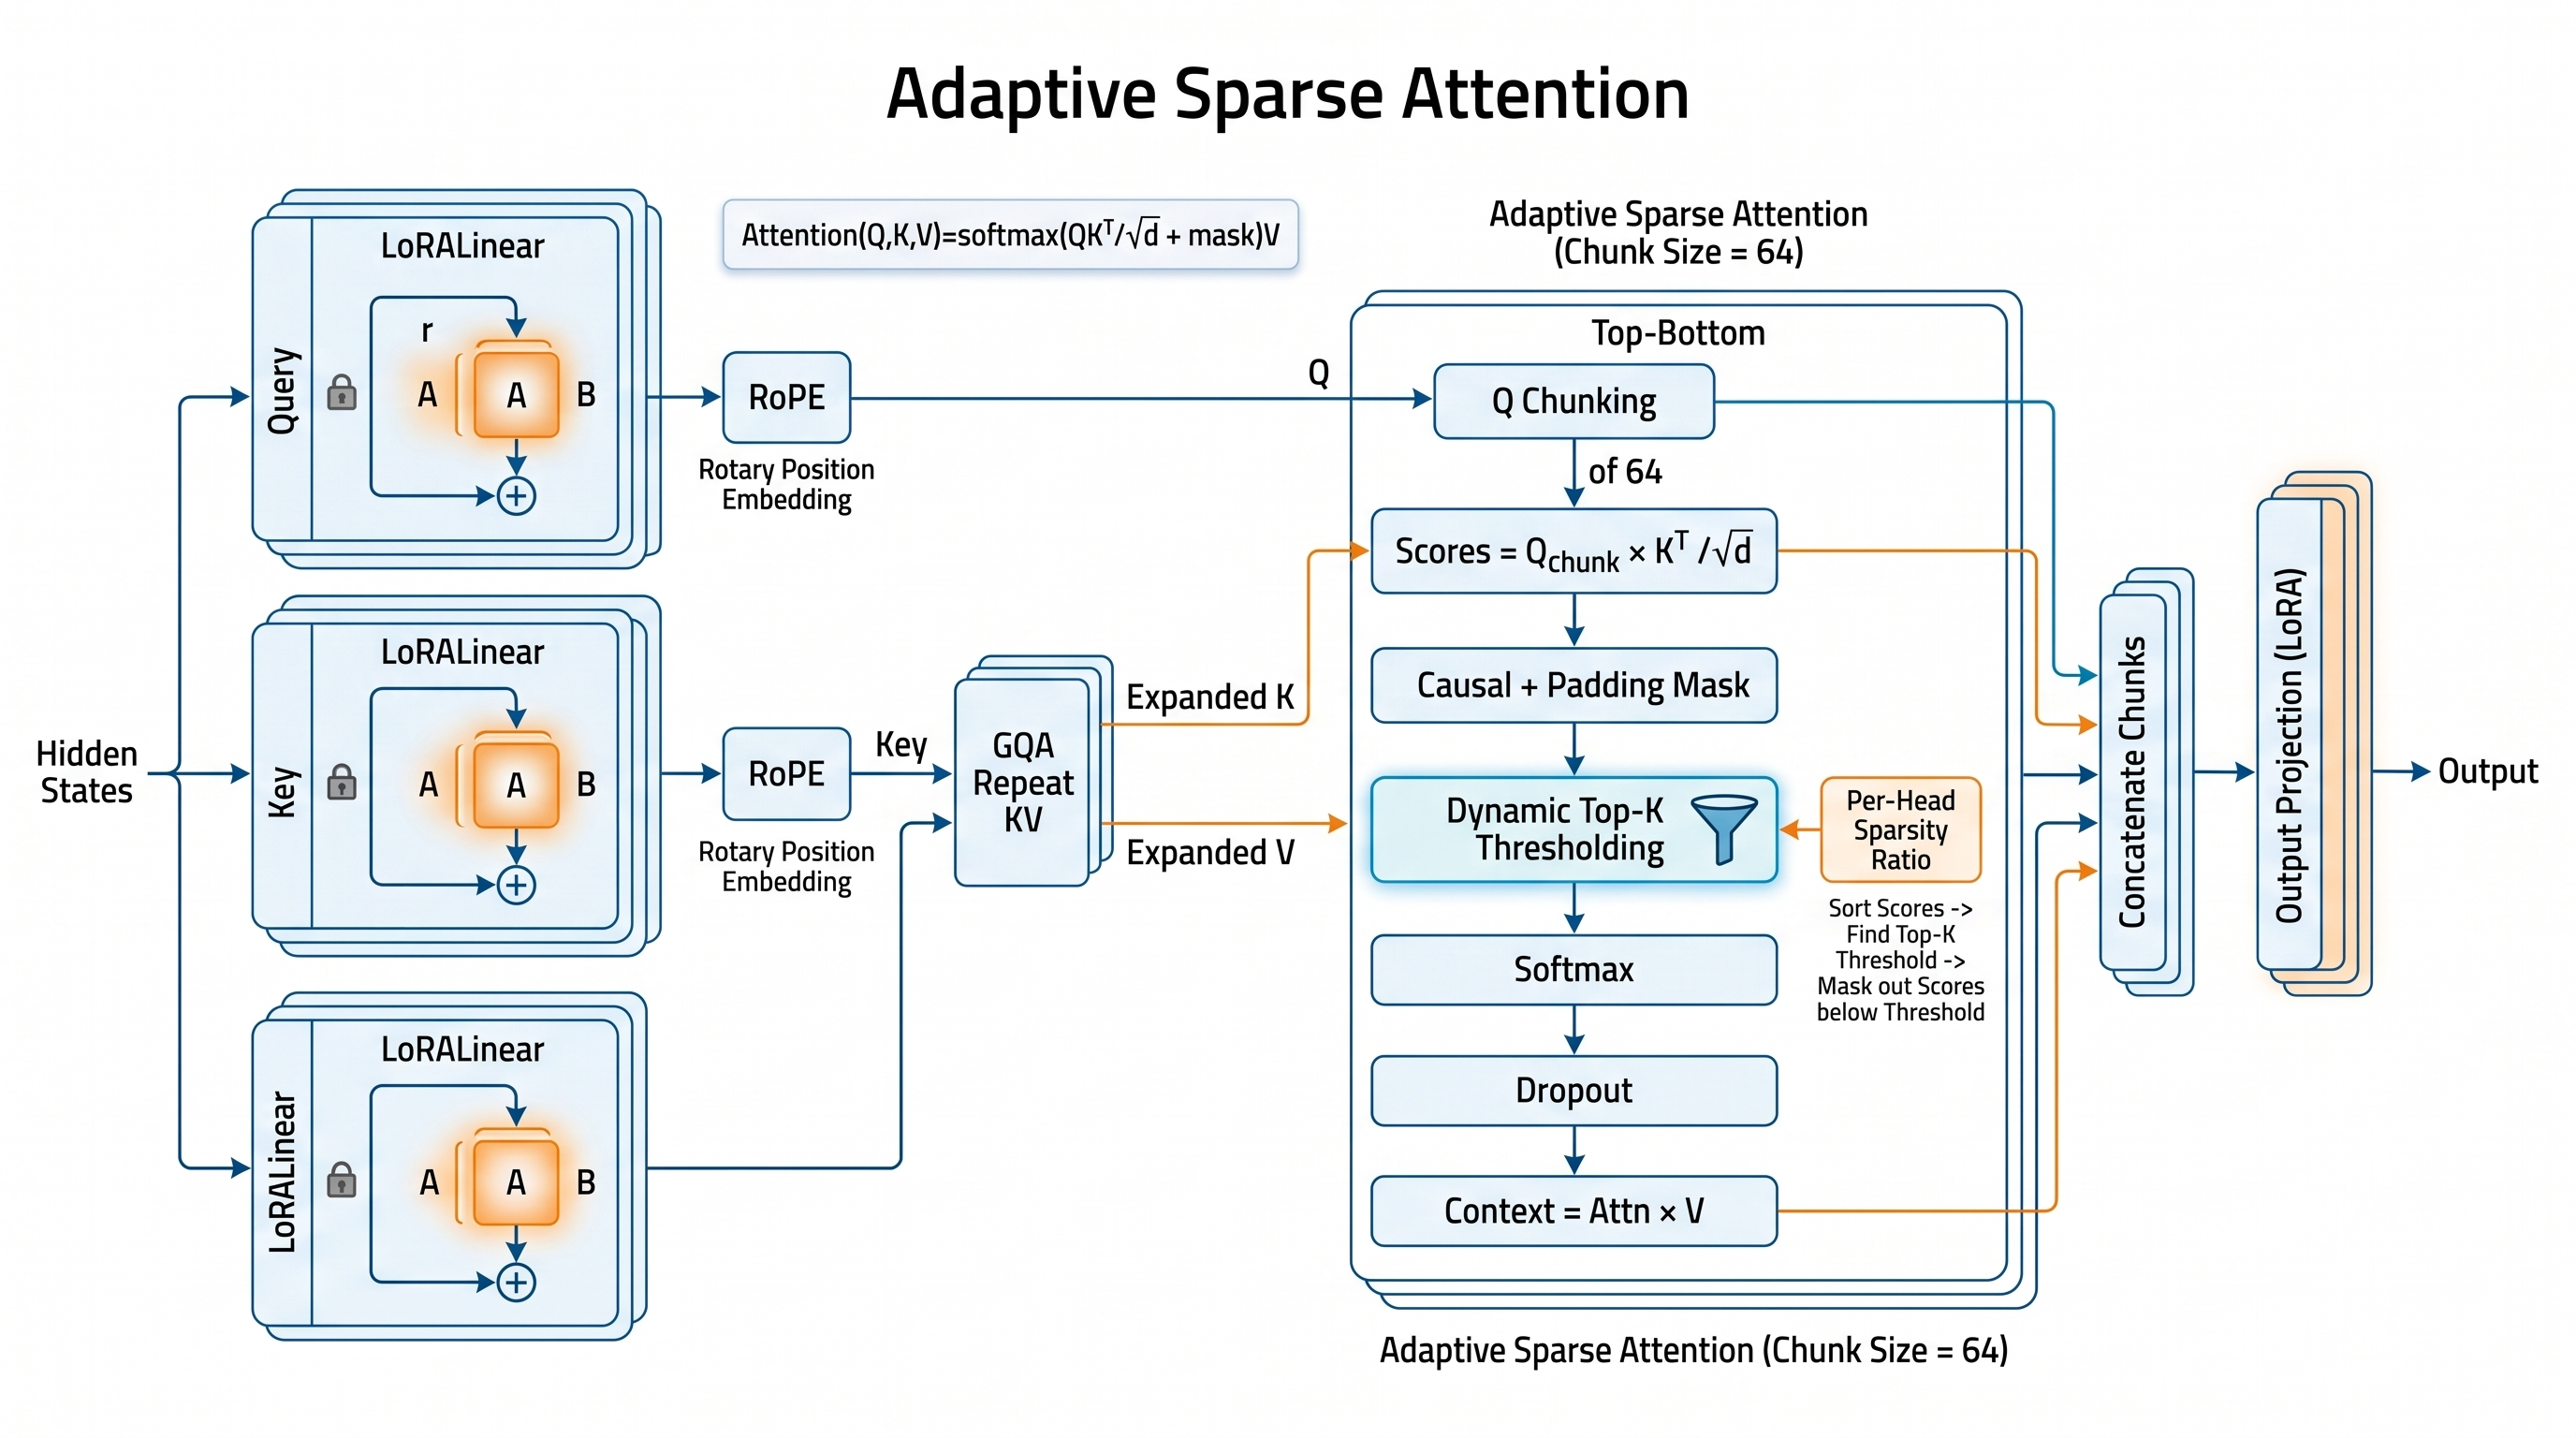
\includegraphics[width=0.92\textwidth]{img/arch_adaptive_sparse_attention.jpeg}
\caption{دیاگرام ساختار معماری و جریان تانسوری ماژول \lr{(adaptive\_sparse\_attention)}}
\label{fig:arch_adaptive_sparse_attention}
\end{figure}

\begin{figure}[H]
\centering
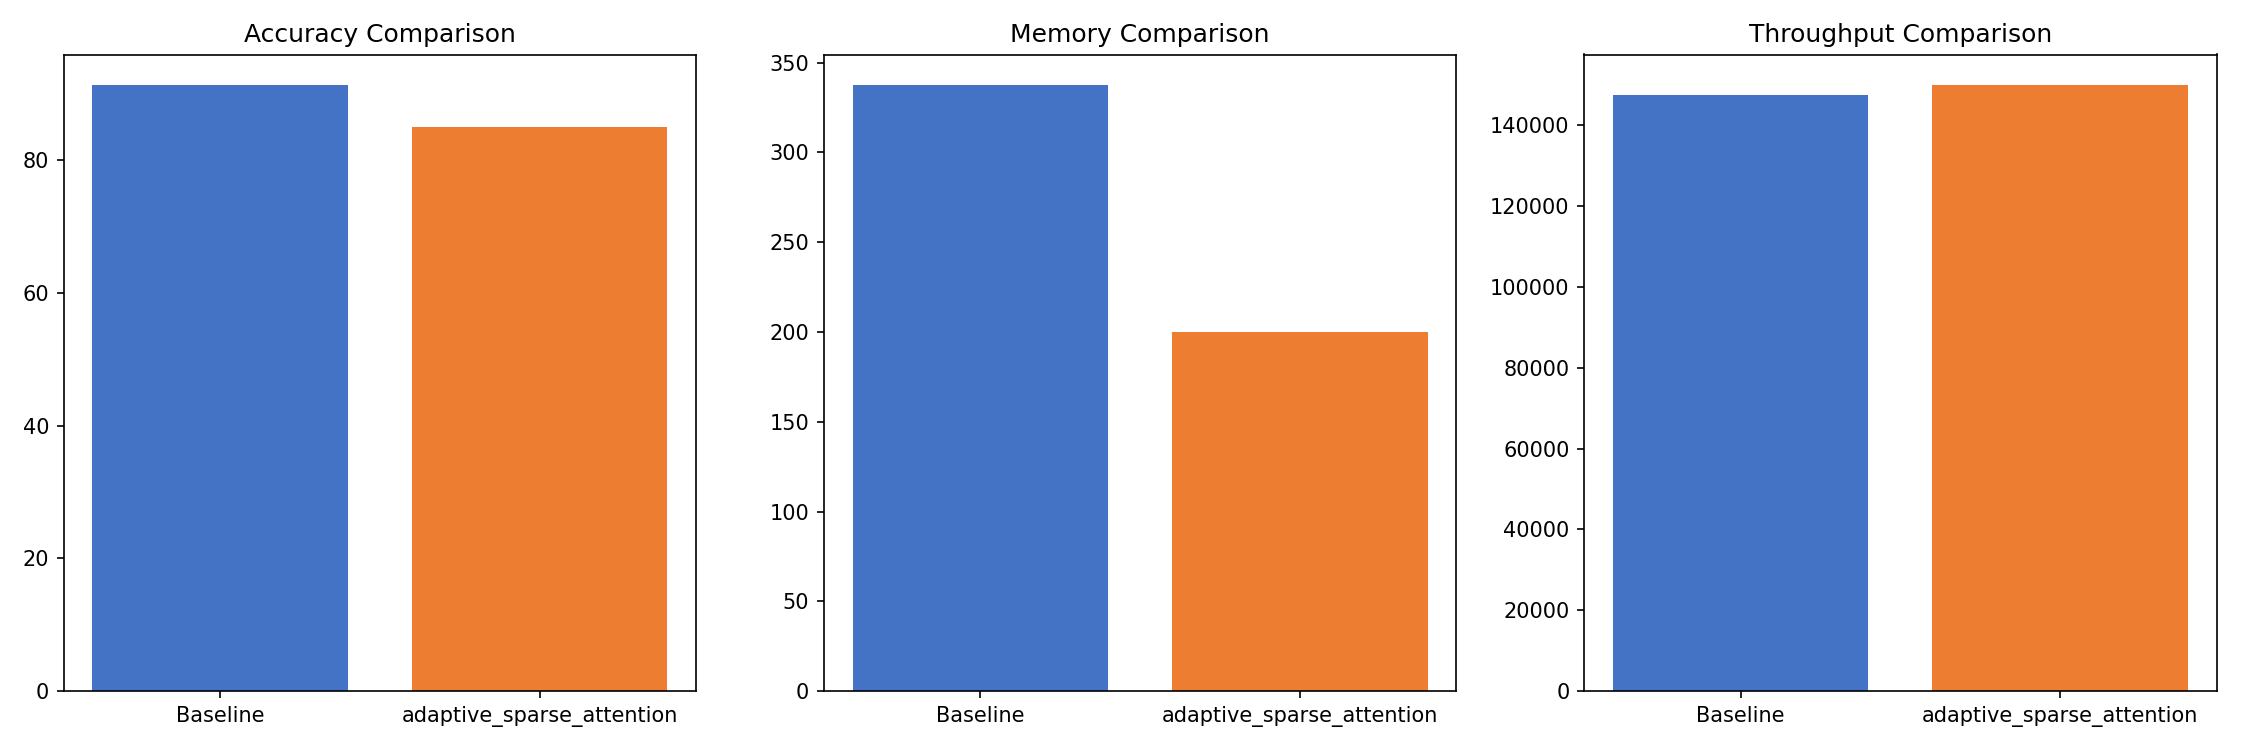
\includegraphics[width=0.92\textwidth]{img/comparison/adaptive_sparse_attention_comparison.png}
\caption{نمودار ارزیابی مقایسه‌ای سه‌شاخصی مکانیزم در برابر خط مبنا \lr{(adaptive\_sparse\_attention)}}
\label{fig:comp_adaptive_sparse_attention}
\end{figure}
